\section{Introduction}
During the requirements gathering process, four distinct components of the system were identified which form a pipeline of execution; \textit{Article Retrieval}, \textit{Keyword Extraction}, \textit{Graph Building} and \textit{Map Drawing}. Crucially, each is specified as being modular, allowing both for flexible extensibility and for alternative implementations to be tested directly against each other without requiring changes to the other components.

This chapter further decomposes these components to provide a detailed overview of the methodology used to implement them, followed by a discussion of the significant challenges and successes which arose during development.

\section{Code Reuse}
I developed the design of the system in Python 2.7 and JavaScript 1.7 using various open-source libraries and APIs for its ancillary functionality. The most notable are detailed below and discussed in context in the following sections.

\begin{itemize}[noitemsep]
	\item\textbf{FeedParser}\footnote{\url{http://pythonhosted.org/feedparser}}: A Python module for downloading and parsing RSS feeds.
	\item\textbf{Newspaper}\footnote{\url{http://newspaper.readthedocs.io}}: A Python library for downloading and extracting content and metadata from online articles.
	\item\textbf{lxml}\footnote{\url{http://lxml.de}}: A Python library for generating, parsing and manipulating XML and HTML.
	\item\textbf{NLTK (The Natural Language Toolkit)}\footnote{\url{http://www.nltk.org}}: A Python library for natural language processing and analysis.
	\item\textbf{Google Knowledge Graph Search}\footnote{\url{https://developers.google.com/knowledge-graph}}: The API for Google's knowledge base, which returns structured semantic search results.
	\item\textbf{D3.js}\footnote{\url{http://d3js.org}}: A JavaScript library for creating and manipulating interactive web visualisations and their underlying data.
\end{itemize}

\section{High-Level Design}
Figure \ref{fig:dfp} outlines the decomposition of the four pipeline into their most important subtasks.

\begin{figure}[htbp!]
	\centering
	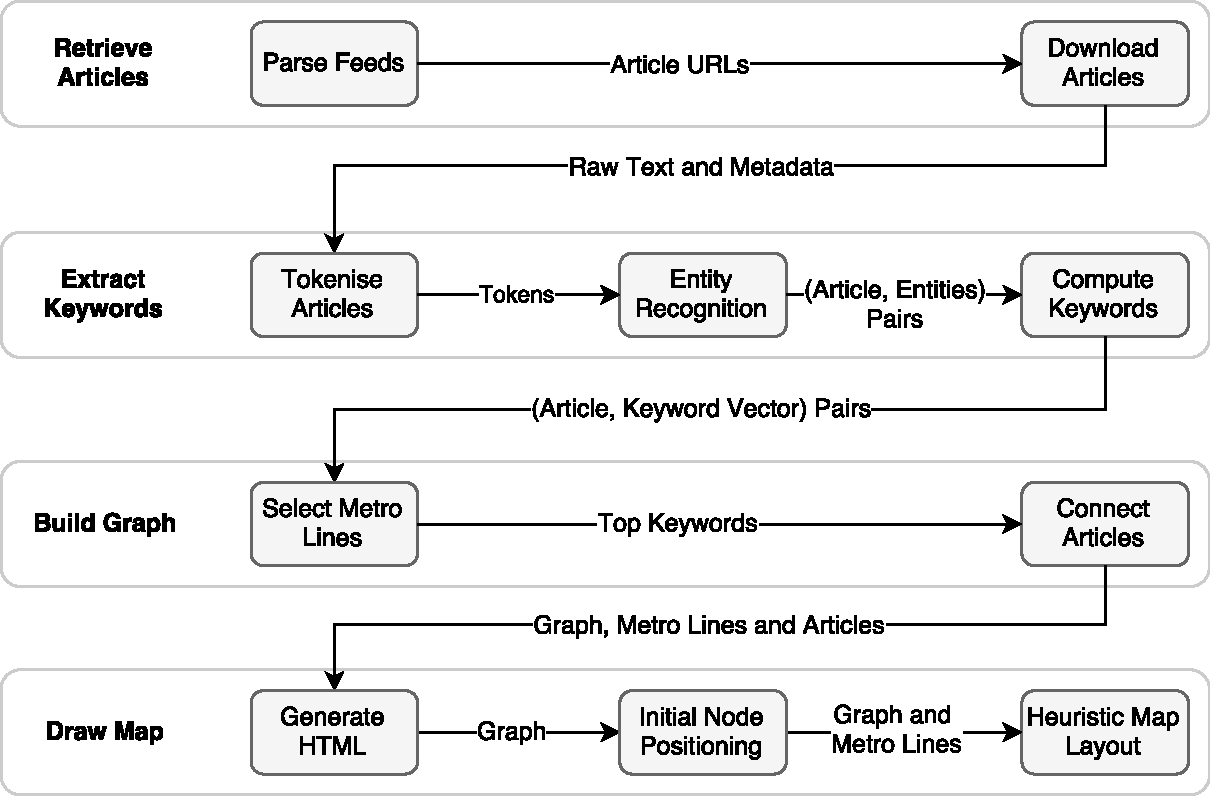
\includegraphics[width=\textwidth]{img/design/DataFlow.pdf}
	\caption{A conceptual model of data flow between components of the system.}
	\label{fig:dfp}
\end{figure}

Not included in Figure \ref{fig:dfp} is the boundary between the \textit{Build Graph} and \textit{Draw Map} stages of the pipeline, which marks the transition from the run-time Python which extracts and processes the article data, to JavaScript which only runs once the visualisation is opened in the browser; the entirety of the  \textit{Draw Map} stage. The boundary takes the form of an intermediate stage between \textit{Build Graph} and \textit{Draw Map}, where the topological map and the article data required for the visualisation are serialised to JSON\footnote{JavaScript Object Notation; \url{http://www.json.org}}.

\section{Article Retrieval}

The first stage of article retrieval is the parsing of RSS feeds, in order for article URLs and metadata to be extracted. The Python library FeedParser was used, as at the time of writing it provided the best support for RSS 0.9x, 1.0 and 2.0. For each item in the feed, the parsing process extracts a link to each article, the name of the channel, and the parsed publish date, but it will also attempt to extract the author name if the \texttt{author} attribute is found.

Once the feed data has been extracted, it is used to construct an instance of \texttt{ArticleCollection}, which acts a wrapper around the contents of one or more feeds and provides the mechanism necessary to perform corpus-wide queries such as calculating inverse document frequency for TF-IDF, and proportional document frequency for TF-PDF. Individual articles are downloaded using the Newspaper library, however due to the requirement that \texttt{ArticleCollection} must be serialisable with cPickle to provide intermediate cache format, it was necessary to create a new \texttt{Article} class which unpacks the necessary members of \texttt{Newspaper.Article} and discards the XML which prevents instances of \texttt{Newspaper.Article} from being serialisable.  The \texttt{Article} encapsulates the functions for computing article-specific terms such as term-frequency for TF-IDF, and the term-weighting component of TF-PDF. 

\subsection{Sanitisation}

An early problem encountered was the embedding of unrelated content into the body of articles by news publishers in order to encourage readers to seek out additional content from the same website. This content typically takes the form of a gallery or list of images and article titles with brief summaries or subheads (see Listing \ref{lst:gallery}).

\begin{HTML}{Unrelated content nested into the body of an article}{lst:gallery}
<div id=`article'>
	<h1> Article Title </h1>
	<p> ... </p>
	<p> ... </p>
	<div id=`gallery'>
		<h1> Related Articles </h1>
		<p> ... </p>
	</div>
</div>	
\end{HTML}

If this content was left and processed as part of an article, it would result in keywords being falsely detected in the articles when in fact they were only present in the form of a link to unrelated content. It was therefore necessary to sanitise the article HTML before tokenisation and keyword extraction. The semantic structure of HTML made this a simpler task; any child elements of the element containing the body text of the article are removed (using lxml) unless they are a paragraph or heading.

The result of this pre-processing stage is an \texttt{ArticleCollection} containing one or more serialisable \texttt{Article}s from one or more RSS feeds, where each \texttt{Article} contains extracted and sanitised but unparsed data, and associated metadata.

\section{Keyword Extraction}

The keyword extraction stage begins with the process of tokenising the body text of every article. Tokenisation here has three substages, all of which were implemented using NLTK (The Natural Language Toolkit for Python), and which are as follows:
\begin{enumerate}
	\item Sentence segmentation: Split the text into a list of sentences and remove sentence punctuation.
	\item Tokenisation: Split each sentence into a list of individual words and remove both whitespace and clause punctuation.
	\item Part-of-Speech (POS) tagging: Categorise each token according to its lexical class, e.g. adjective. This more of an extension to the tokenisation process than a part of it, but it is performed directly after tokenisation and is necessary for the next stage of processing.
\end{enumerate}
\begin{figure}[htbp!]
	\centering
	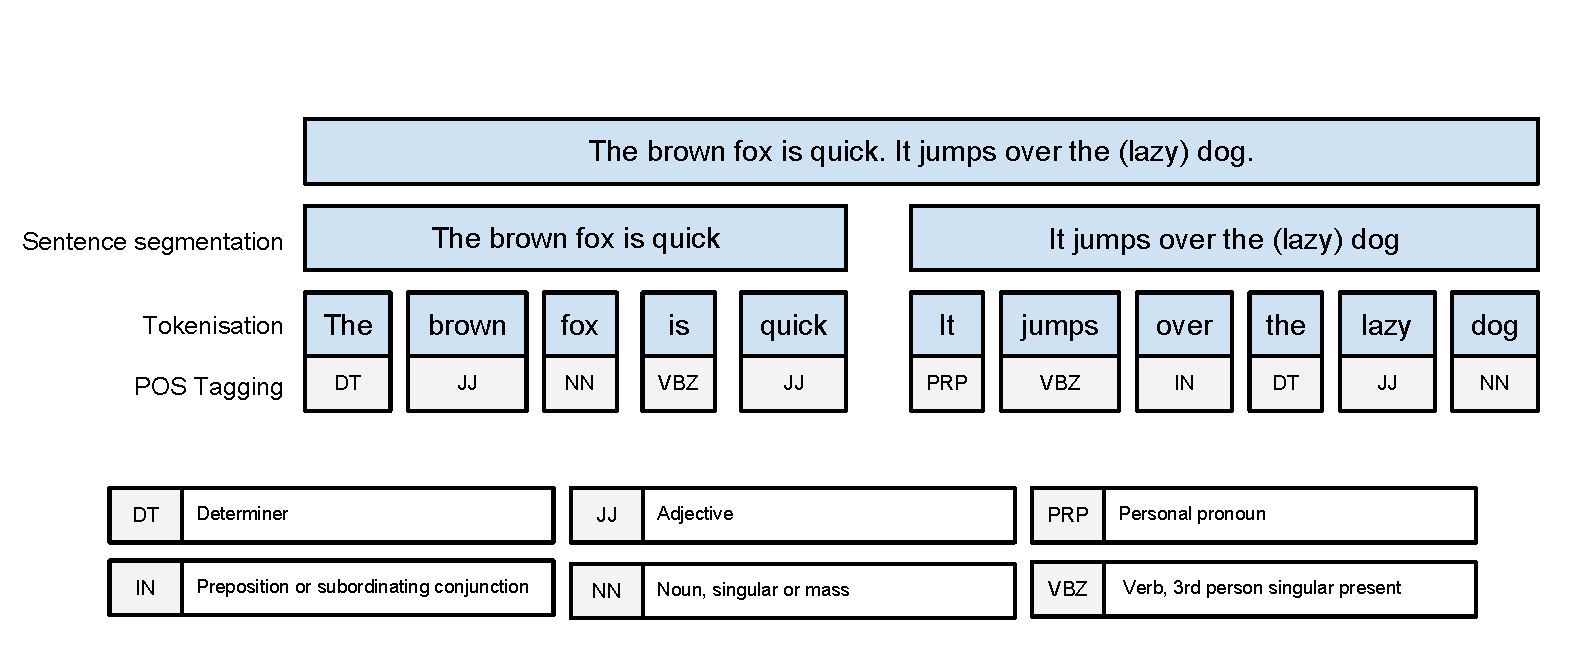
\includegraphics[width=\textwidth]{img/implementation/Tokenisation.pdf}
	\caption{Stepping through the tokenisation process}
	\label{fig:tokenisation}
\end{figure}

\subsection{Named Entity Recognition}

The second half of the keyword extraction process is exclusively concerned with named entities within articles. This is because, intuitively, the names of people, places, events companies and other \textit{things} form a set of strong candidate keywords. Restricting the candidates to entities alone reduces the search space by an order of magnitude when using frequency-based methods for keyword extraction, and bypasses the need for other natural language processing tasks such as stop-word removal and lemmatisation.

Once tokens have been POS tagged, named-entity chunking can be performed, again using NLTK. This process groups tokens into contiguous and non-overlapping \textit{chunks}, where each chunk is a named entity; typically a proper noun or some other noun phrase.

It is possible for chunks to contain other chunks (consider the chunk `Bank of England', which contains the chunk `England'), but this is typically undesirable for entity recognition -- where we desire specificity -- so after chunking the tokens, we flatten the chunk structure so chunks cannot be any further decomposed.

At this stage, we have a list of chunks, each of which will be an eventual candidate for becoming a metro line. However, the chunks require some further processing before we can determine whether or not they are significant keywords.

\subsubsection{Name Disambiguation: Substring Matching}
It is common stylistic practice in journalism to refer to the subjects of articles by their surnames. However, to avoid any confusion, the full names of those mentioned will often appear in the title or first few paragraphs of the article. If keyword strength is determined by frequency, then regardless of whether we use TF-IDF or TF-PDF, we need every occurrence of an entity to refer to that entity by the same name; preferably the most specific, which is typically the longest.

During name disambiguation, we only consider entities with more than one mention in the source text as candidates. This is because the chunking process can produce false positives by combining unrelated adjectives with valid chunks, but the likelihood of the same false positive being produced twice or more in the same article is low.

Let $P$ denote the set of entities with more than one occurrence in the source article; $S$:
\begin{align*}
P &= \{e\;|\;\text{occurences}(e, S) > 1\}.
\intertext{$\forall (e_1, e_2) \in \{P\times{P}\;|\;$length$(e_1)\;<\;$length$(e_2)\}, $ if $e_1 $ is a substring of $e_2$, we call $e_1$ an \textit{alias} of $e_2$. Let $A$ be the set of alias pairs in $S$;} 
A &= \{(a, e) \;|\;a \text{ is an alias of } e\}
\intertext{We require the first term of every pair in $A$ to be unique, but there is no such constraint for the second term ($e$); this allows multiple aliases to map to the same entity. For example,} 
 & \{(\text{`Zuckerberg'}, \text{`Mark Zuckerberg'}), (\text{`Zuck'}, \text{`Mark Zuckerberg'})\} 
%\intertext{and}
%& \{(\text{`Zuck'}, \text{`Zuckerberg'}), (\text{`Zuckerberg'}, \text{`Mark Zuckerberg'})\}
\intertext{would be unambiguous and therefore valid, but}
 & \{(\text{`Mark'}, \text{`Mark Zuckerberg'}), (\text{`Mark'}, \text{`Zuckerberg'})\}
\intertext{would not be. Let $U$ be the set of unambiguous alias-entity pairs in $S$:}
U &= \{(a, e) \;|\; (a, e)\in{A} \cap \forall(e_1, e_2)\in A, \; a = e_1 \implies e = e_2 \}
\end{align*}

We have a reasonable degree of confidence that for every alias-entity pair $(a, e) \in U$, occurrences of $a$ in the source text can be replaced by $e$, making $e$ a stronger candidate for keyword detection. Pairs in $(a, e) \in A\setminus{U}$, that is, aliases which could map to multiple entities in the source, are disregarded at this stage and left unchanged. A more sophisticated method of name disambiguation could address this.

Algorithm \ref{alg:u} illustrates how, given a list of entities, we can find the unambiguous pairs deterministically in $\mathcal{O}(n^2)$ time. 

\begin{algorithm}
\label{alg:u}
 \caption{Finding unambiguous alias-entity pairs}
 \KwData{$names$: a list of recognised entities}
 \KwResult{$U$: the set of unambiguous pairs in $names$}
 $U \Leftarrow$ \{\}\;
 \ForEach{$e_1, e_2$ $\in ($names $\times$ names$)$}{
   \If{len($e_1$) $>$ len($e_2$)}{
   	swap($e_1$, $e_2$)\;
   }
  \If(\tcc*[f]{If $e_1$ is a substring of $e_2$}){$e_1 \in e_2$}{
   	\eIf{$e_1 \notin U$}{
   	  $U$[$e_1$] $\Leftarrow e_2$ \tcc*[r]{$(e_1, e_2)$ are a candidate pair}
    }{
      delete $U$[$e_1$] \tcc*[r]{$e_1$ is now ambiguous, so remove it}
    }
   }
 }
\end{algorithm}


\subsubsection{Entity Disambiguation}

Entity disambiguation describes the process of determining the identity of entities in a body of text. Performing this process on the sentence `The UK has voted to leave the EU,' should identify `UK' as The United Kingdom and `EU' as The European Union. As advanced methods for entity disambiguation are both complex and computationally expensive, I did not attempt to implement a formal method for this. 

Instead, the list of recognised entities are queried against Google's publicly accessible Knowledge Graph API, which returns a list of potential results as Schema.org\footnote{http://schema.org is an online hierarchy of types managed by W3C (The World Wide Web Consortium)} types. Knowledge Graph is the service which replaced Freebase in 2015, and currently contains over 70 billion facts \citep{knowledgegraph}.

Each result has a score attributed to it by Knowledge Graph, which is an indicator the strength of the match between the entity and the original query. Results are sorted by descending score; the higher the \texttt{resultScore}, the better the match. Although there is no defined upper limit for this value, comparing the scores of the top two results for a query can provide a measure of certainty, for all but particularly esoteric or unknown entities.

We specify a threshold $\frac{1}{t}$, which is roughly proportional to the likelihood of accepting a false positive match. Then, if dividing the score of the first result by the score of the second yields a number greater than $\frac{1}{t}$, we accept the match. Provisionally we set $t=0.5$; a discussion of how I arrived at this value is provided in the next section.

Using a knowledge base for disambiguation also inadvertently solves another problem I encountered while parsing articles, this time as a result the expositional style of journalistic writing. While keywords are typically nouns or noun phrases, they can also appear in the form of denominal adjectives. These adjectives are derived from nouns; e.g. `French' implies `France' might be a keyword. Denominal adjectives are not amenable to traditional stemming or lemmatising, but querying Knowledge Graph for `French' returns a top match of `France' with a \texttt{resultScore} of 432.42807; more than four times larger than the next result.

Given a list of entities $E$, and top two results of a Knowledge Graph query for each $e \in E$; $R_e(1)$ and $R_e(2)$ with scores $S_e(1)$ and $S_e(2)$ respectively, our aim is to return a set of pairs mapping zero or more entities in $E$ to their disambiguated forms;

\begin{align*}
K &= \bigg\{(e, R_e(1))\;|\;\frac{S_e(1)}{S_e(2)} > \frac{1}{t}\bigg\}
\end{align*}

Algorithm \ref{alg:kg} describes this process. For higher values of $t$, the likelihood of accepting a false positive increases, and for lower values, the likelihood of accepting a false negative increases. For corpora which do not contain references to public figures and place names, choice of $t$ should be empirically tuned against the prevalence of the expected entities.

\begin{algorithm}
\label{alg:kg}
 \caption{Entity disambiguation with Knowledge Graph}
 \KwData{$names$: a list of recognised entities \\ 
 		\hspace{1.2cm}$t$: the acceptance threshold for results, default = 0.5}
 \KwResult{$K$: a set of disambiguation mappings for elements in $names$}
 $K \Leftarrow$ \{\}\;
 $T \Leftarrow 1\div{t}$\;
 \ForEach{$e \in names$}{
 	$results \Leftarrow$ KnowledgeGraphResults($e$)\;
 	\If{len($results$) $>$ 1}{
	   \If{$results$[0].score $\div$ $results$[1].score $> T$}{
	   		$K[e] = results[0].name$\;
	   }
	}
 }
\end{algorithm}

It is unclear what should become of queries that Knowledge Graph only returns a single result for, but in this implementation they are ignored.

\subsubsection{Determining Optimal Values for $t$}

Empirically, I found the best values for $t$ are in the range $0.35 < t < 0.65$, meaning we accept top results which are at least 1.5x-3x higher than the next best candidate. To determine this, I logged all the disambiguation pairs found in 20 articles from the BBC Politics RSS feed, letting $t$ range over \{0.3, 0.5, 0.7, 0.9\}. I then manually classified the pairs as either true or false positives. 

Figure \ref{fig:dthreshold} shows the results of this investigation, with total pairs plotted alongside the percentage of those pairs which were false positives.\footnote{Since it is both extensive and tangential to the focus of the project, raw data for this table can be found at \url{http://bit.ly/DisambiguationThresholding}.} Although we see a reduction in false positives for smaller values of $t$, the trend-line illustrates that this is a game of diminishing returns; reducing $t$ from 0.3 to 0.1 only reduces the false positives by 4.34\%, but it leads to 43 fewer pairs being identified. 

There is a clear trade-off between the accuracy of the disambiguation and the number of false negatives we discard, but the cost of false positives in this case is less than the cost of false negatives. While a false positive could result in unrelated entities appearing as keywords for certain articles, the likelihood of the same false positive appearing with high frequency in enough articles to result in an erroneous metro line is incredibly low. In contrast, the cost of disregarding a false negative could result in articles being left off certain metro lines altogether. It is for this reason that we don't simply choose the value of $t$ which yields the minimum ratio of false positives.

\begin{figure}[htbp!]
	\centering
	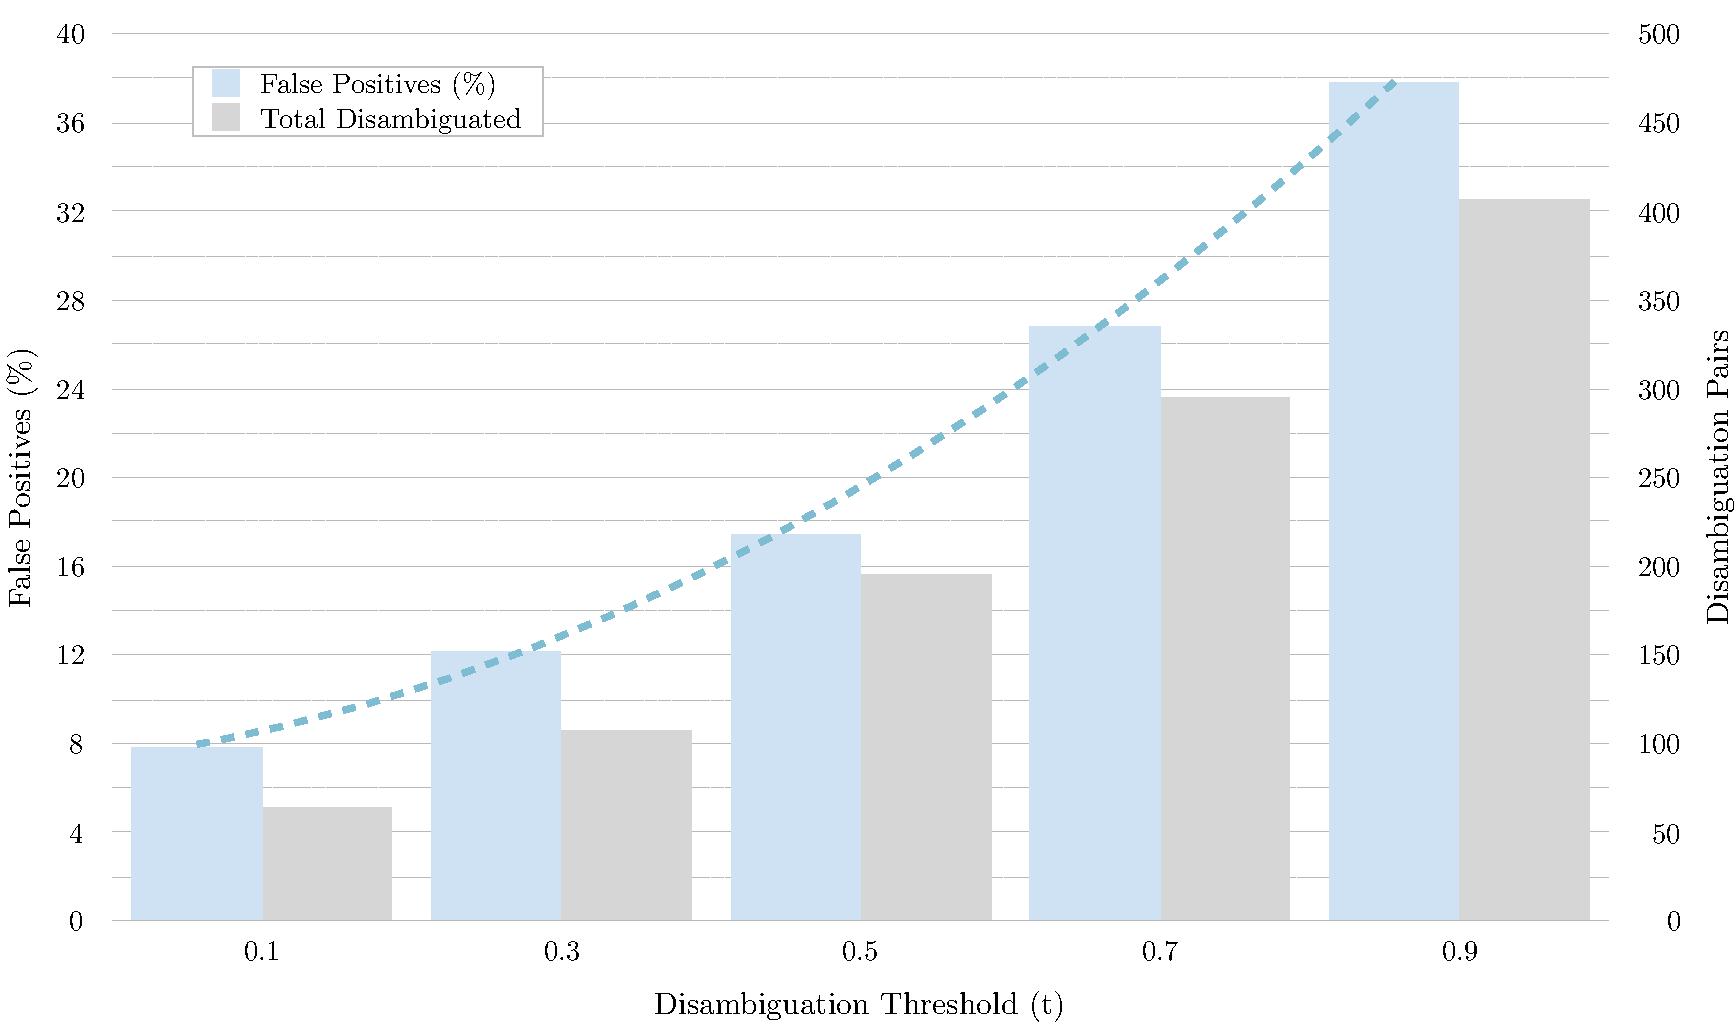
\includegraphics[width=\textwidth]{img/implementation/DisambiguationThreshold.pdf}
	\caption{Disambiguation threshold against pairs found and false positives (\%)}
	\label{fig:dthreshold}
\end{figure}



\subsection{Keyword Ranking}

Given a set of disambiguated entities for every article, the union of which forms a set of candidates keywords or \textit{metro lines} for the collection, we must now determine which keywords are the most relevant. To do this, the two methods described in Chapter \ref{c:litreview} will be revisited; TF-IDF \citep{tfidf} and TF-PDF \citep{TopicExtractionfromnewsArchiveUsingTFPDFAlgorithm}. Both were implemented in the system so they could be compared directly against each another.

From an implementation perspective, the main difference between these two algorithms are the level at which they operate. TF-IDF is calculated on a per-article basis, returning a vector of an article's keywords and their corresponding scores.

%\begin{itemize}[noitemsep]
%	\item $d$ = The contents of the document containing $t$;
%	\item $C$ = The background corpus, which contains one or more documents;
%\end{itemize}
%
%\begin{equation}
%	\text{TF-IDF}(t) = \frac{Occurrences(t, d)}{WordCount(d)} \times log_e\bigg(\frac{|C|}{|\{c \in C \mid t \in c\}|}\bigg)
%\tag{\ref{eqn:tfidf}}
%\end{equation}

In contrast, TF-PDF is specified at corpus level, where there are one or more channels within the corpus. In our case, channels can be conveniently defined as RSS feeds, to correct the bias which could arise from all articles within a channel containing a specific keyword which is then identified as significant due to the relatively small size of that channel against the rest of the corpus. Similarly to TF-IDF however, it produces a vector of pairs of keywords and their scores.

%\subsubsection{Implementation of TF-PDF Vectorisation}
%
%\begin{itemize}[noitemsep]
%	\item $D$ = The number of channels in the corpus;
%	\item $K_c$ = The total number of terms in channel $c$;
%	\item $F_{tc}$ = Frequency of term $t$ in channel $c$;
%	\item $n_{tc}$ = The number of articles in channel $c$ where term $t$ occurs;
%	\item $N_c$ = The total number of articles in channel $c$.
%\end{itemize}
%\begin{equation}
%	\text{TF-PDF}(t) = \sum_{c=1}^{c=D}\frac{F_{tc}}{\sqrt{\;\sum\limits_{k=1}^{k={K_c}}{F_{kc}}^2}}\times\text{exp}{\bigg(\frac{n_{tc}}{Nc}\bigg)}
%\tag{\ref{eqn:tfpdf}}
%\end{equation}

For both equations, the advantage to restricting the set of candidates to named entities is apparent. Figure \ref{fig:tokensentities} shows the number of tokens against the percentage of extracted entities for 40 articles from the BBC's Politics RSS Feed.\footnote{http://feeds.bbci.co.uk/news/politics/rss.xml (Accessed: 27/02/2017, Full data in Appendix \ref{tab:entitiestokens})} The interquartile range is shown, illustrating that 50\% of articles had entities comprising 5.4\%-8.2\% of their tokens after stop-word removal. With the mean equal to 6.65\%, the implications of this are a search space which can be reduced by a factor of more than ten. Although performance optimisation was not specified in the aims of the project, gains of this nature are still significant.

\begin{figure}[htbp!]
	\centering
	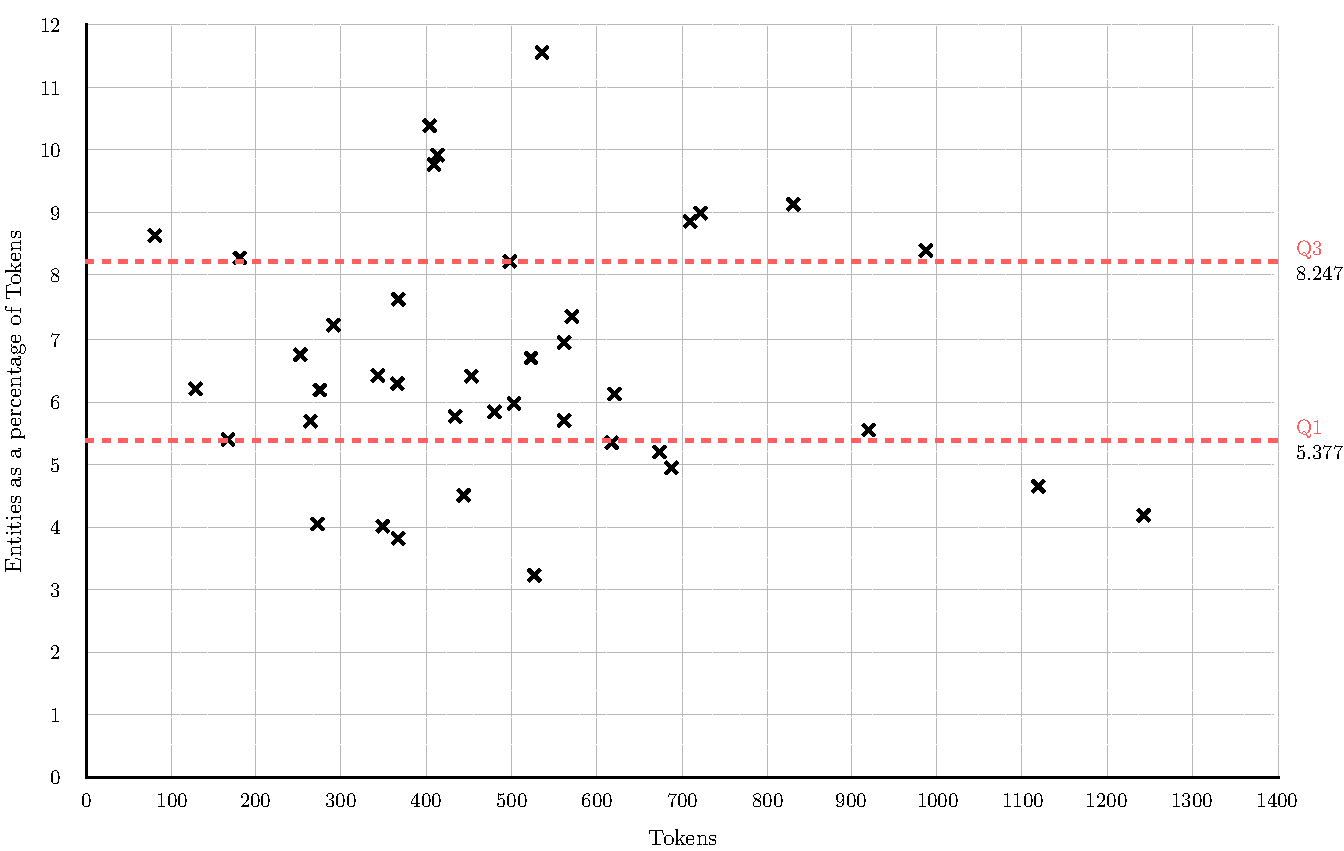
\includegraphics[width=\textwidth]{img/implementation/TokensEntities.pdf}
	\caption{Entities as a percentage of Tokens across 40 BBC Politics articles.}
	\label{fig:tokensentities}
\end{figure}



\section{Graph Building}

\subsection{Choosing Lines}

\subsection{Connecting Articles}

\section{Map Drawing}

\subsection{Initial Node Positioning}
\begin{itemize}[noitemsep]
	\item D3.js for force directed layout
	\item Initial force parameters; adjusting based on \cite{AutomaticMetroMapLayoutThesis, AutomaticMetroMapLayout}
\end{itemize}

\subsection{Heuristic Layout}
\begin{itemize}[noitemsep]
	\item \cite{AutomaticMetroMapLayoutThesis, AutomaticMetroMapLayout} for snap()
	\item Repeated averaging along lines for sensible octilinearity
	\item Straightening the ends of lines
\end{itemize}
